\documentclass[../rapport.tex]{subfiles}
\graphicspath{{\subfix{ressources/photos_diagrammes/app2/}}}

\begin{document}

\begin{figure}[h!]
	\centering 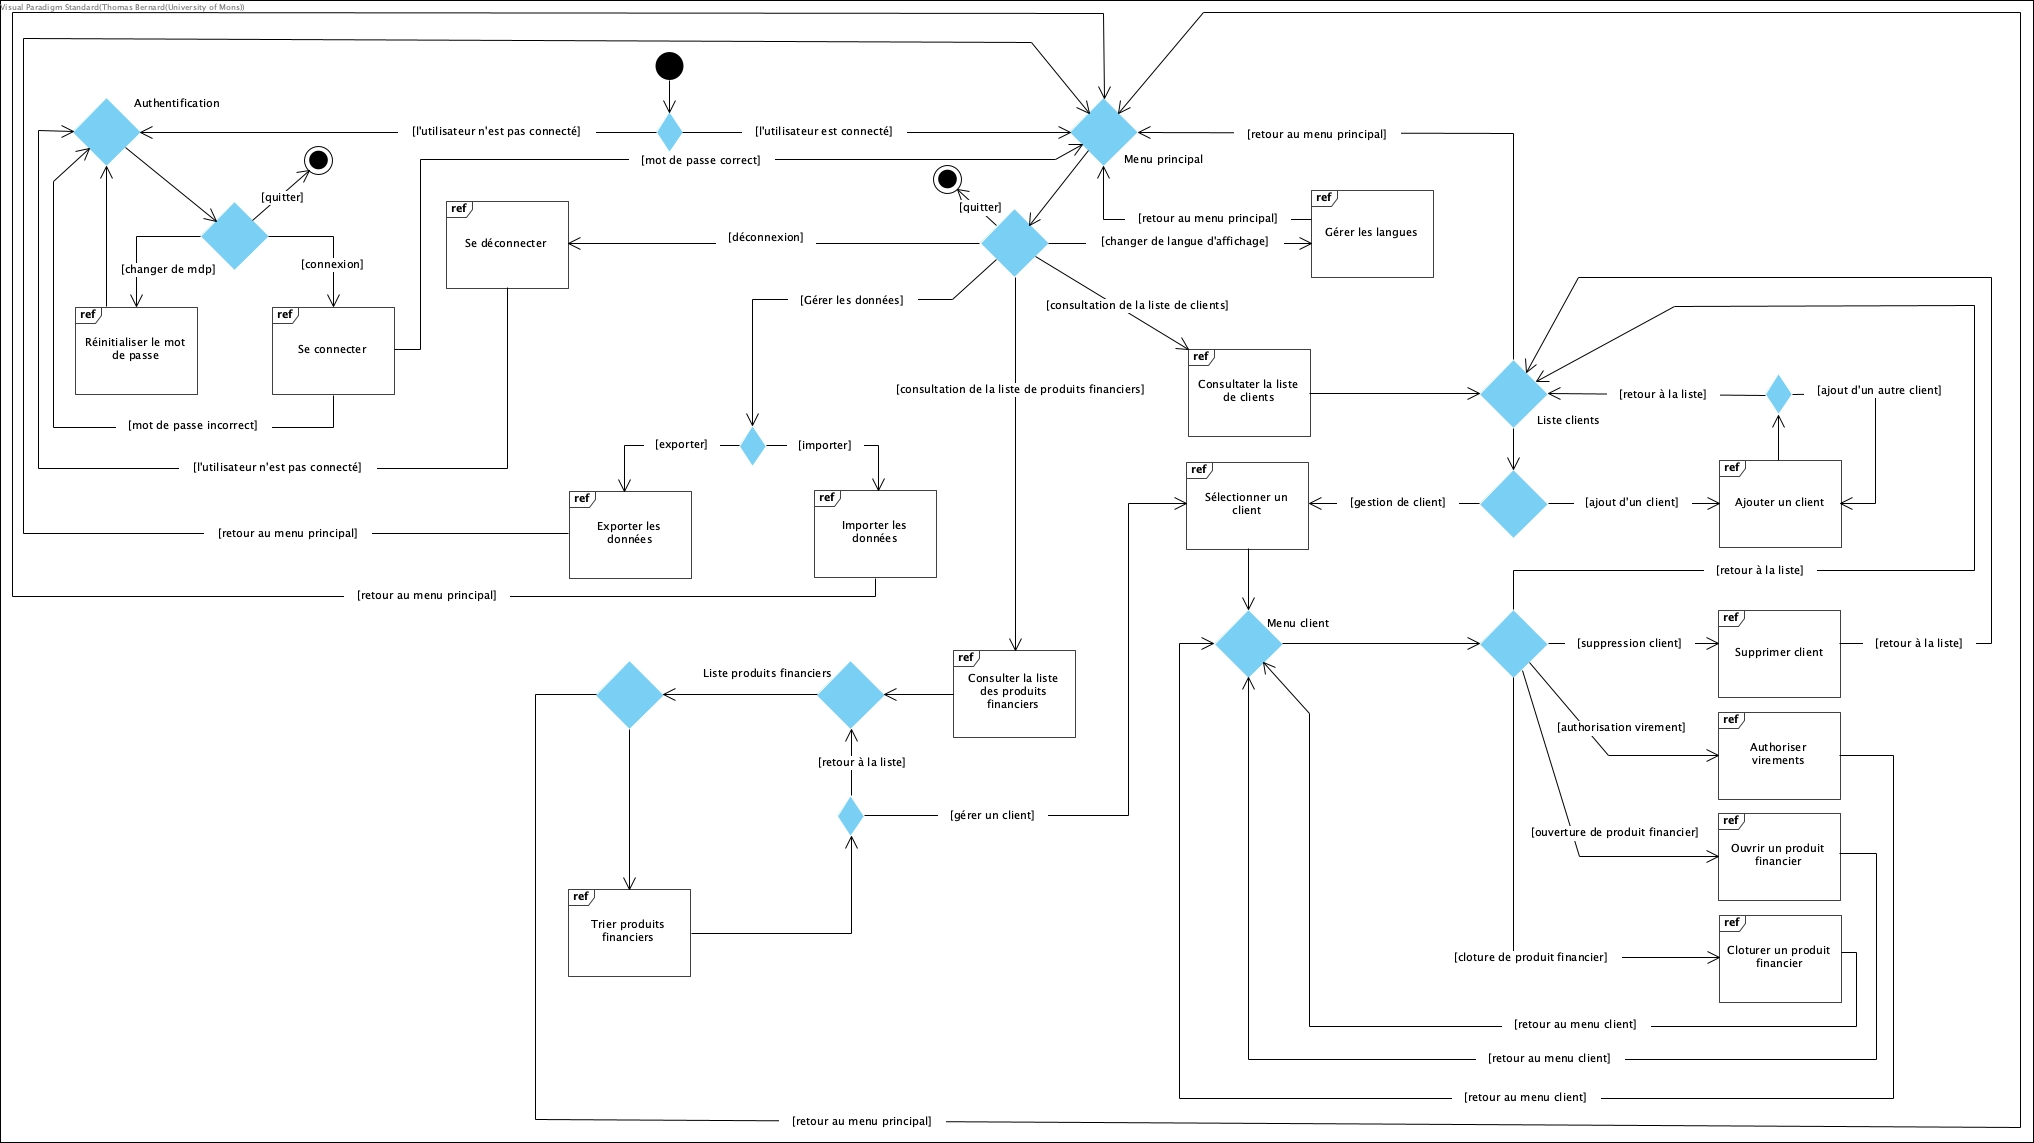
\includegraphics[scale=0.20]{ressources/photos_diagrammes/app2/int_over_app2.jpg}
	\caption{Interaction Overview Diagram Application 2.}
\end{figure}

L'utilisateur d'un application d'institution financière devra d'abord s'authentifié via le menu d'authentification schématisé dans le coin supérieur gauche du diagramme.\\
Il devra utilisé le numéro swift et mot de passe de l'institution pour laquelle il travaille. Il pourra ensuite choisir de rester connecté à l'application.\\
Le menu principal de l'application permet d'accéder à la liste des clients et ainsi depouvoir effectuer des opérations sur chaque client de l'institution ou d'en ajouter de nouveaux.\\
La partie gestion de clients est schématisée dans la partie droite du diagramme.

\end{document}
